\subsection*{Castillo de Cornelia}
A continuación, se muestra un mapa de la planta baja, donde los lugares importantes llevan el número de su párrafo correspondiente. Las escaleras del centro conducen a la sala de trono, mientras que la entrada del fondo conduce al palacio, que se encuentra actualmente cerrado. El palacio está lleno de guardias armados en todo momento.
\begin{center} 
	\tcbox[left=0pt,top=0pt,right=0pt,bottom=0pt, boxsep=0pt, colframe=accent, sharp corners]{
		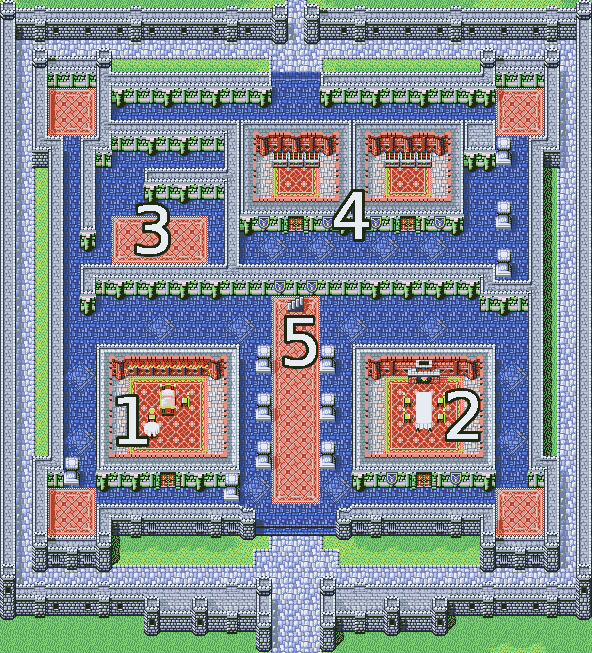
\includegraphics[width=0.98\columnwidth]{./art/maps/castle.png} 
	}
\end{center}
\subsubsection*{1 Habitación de la reina}
"Por favor… devuélvanme a mi hija… a mi Sarah… sana y salva".
\indent -- Reina Jayne \\\\
La reina Jayne es una mujer de mediana edad con pelo turquesa y ojos azules, un vestido largo y rojo y una tiara dorada. Ha estado muy deprimida desde el secuestro de su hija y solo habla con el grupo después de que se han ganado la confianza del rey. En la conversación, les da detalles al grupo sobre la noche del secuestro, el cual ella ha presenciado personalmente. En esa noche, despertó y encontró a Garland escapando con la princesa inconsciente en sus brazos. Garland le dijo que si quería volver a ver a su hija viva, debía entregar el control del reino de Cornelia. Después desapareció con Sarah por la entrada trasera del palacio. La reina está traumatizada por este acontecimiento y se culpa por no haber e el secuestro. 

\subsubsection*{2. Habitación de la hermana}
"M-m-mi hermana… ¿D-d-dónde está mi hermana?"\\
\indent -- Alison\\\\
Esta es la habitación de Alison, la hermana de Sarah Es una adolescente sensible que se parece mucho a su madre. Los guardias que custodian su puerta dicen al grupo que Alison se encerró y no quiere abrir la puerta. Si el grupo puede convencerla (por ejemplo, declarando que ellos salvarán a Sarah), ella abrirá la puerta para hablar con ellos. Alison conoce bien a su hermana, ya que la admira mucho. Le cuenta al grupo que Sarah siente una gran pasión por la música y que su preciado laúd ha desaparecido junto con ella. Si el grupo consigue calmar a Alison, tienen más probabilidad de convencer al rey, que está preocupado por ella. 

\subsubsection*{3. Capitán}
"Garland alguna vez fue el mejor caballero del reino. Pero el poder lo ha corrompido y se alejó de su propia naturaleza".
\indent -- Ian \\\\
El capitán de la guardia es un hombre joven de pelo largo y rubio llamado Ian. Lleva una armadura pesada decorada y una espada larga en la espalda. Es reacio a hablar de los aventureros. El grupo advierte de inmediato que le falta el brazo izquierdo. Si el grupo ha convencido al rey, el capitán está dispuesto a hablar con ellos sobre la fallida misión de rescatar a Sarah, que él mismo dirigió. Justo después de que Sarah desapareciera, sus hombres siguieron Garland y lo enfrentaron en el Gran Puente, al norte de Cornelia. Sin embargo, Garland los superó a todos en combate y el capitán fue el único sobreviviente, aunque perdió un brazo. Está avergonzado por su fracaso y se ve profundamente perturbado y asustado del poder de Garland. 

\subsubsection*{4. Sala del tesoro}
La Sala del tesoro consta de dos habitaciones: la de la izquierda contiene el oro del palacio, mientras que la derecha contiene equipos y objetos caros. Ambas puertas están protegidas por dos hombres bien armados con armaduras pesadas. Si el grupo ha obtenido una carta del rey, se le entregan los siguientes objetos: Una Carpa lo suficientemente grande para todo el grupo. También reciben una poción y 200 Gil cada uno. 

\subsubsection*{5. Sala del trono}
La puerta está protegida por dos guardias reales armados con gujas y armadura pesada decorada. Dentro de la sala, el rey está en su trono y al lado de él se encuentra el canciller. El rey es un hombre de mediana edad con ojos azul claro, de cabello castaño y una barba larga. Lleva una corona dorada y una larga túnica roja. El canciller es un poco más joven, tiene pelo oscuro y también lleva ropas de noble. El rey está encantado de ver a los aventureros, ya que está desesperado por encontrar a su hija, pero el canciller se muestra muy escéptico. En la siguiente conversación, el grupo puede intentar convencer al rey de que puede rescatar a Sarah, pero el canciller convence al rey de que antes tienen que demostrar que son dignos de confianza. A continuación, el rey lamenta que ha abandonado a su pueblo por concentrarse en el rescate de su hija. Pide al grupo que ayude a las personas de Cornelia para que demuestren que son capaces de salvar a Sarah. A cambio, les promete proporcionarles suministros para el viaje. Si el grupo pide más detalles sobre el secuestro, no revelarán nada más hasta que el grupo haya ganado su confianza. 

\subsubsection*{Convenciendo al rey}
"Garland ya no es el hombre que yo conocí… Se los suplico. ¡Devuélvame pronto a mi hija!"

\indent -- Rey de Cornelia \\\\
Para convencer al rey, el grupo tiene que cumplir una serie de tareas que ayudan a las personas de Cornelia, el DJ decide a quiénes y la cantidad. A continuación se muestra una lista de tareas que pueden convencer al rey si se cumplen:
\begin{itemize}[leftmargin=*]
	\item Ayudar al herrero a recibir su mercancía.
	\item Resolver una disputa entre los dos magos.
	\item Defender el puerto de un ataque de piratas.
	\item Ayudar a la capilla a recuperar a sus fieles.
\end{itemize}
Una vez que el grupo gana la confianza del rey, él les revela más detalles sobre el secuestro: Sarah fue secuestrada por un excaballero de Cornelia llamado Garland, el espadachín más poderoso del reino. Garland era muy cercano al rey, pero el poder lo corrompió y exigió ser el sucesor del rey. Cuando el rey se lo negó, Garland secuestró a su hija Sarah, exigiendo el control del reino de Cornelia como pago por su rescate. Muchos otros caballeros han intentado salvarla desde entonces y aunque ninguno ha tenido éxito, descubrieron que Garland tiene cautiva a Sarah en el Santuario del Caos, al norte de Cornelia, pasando el Gran Puente. El rey cumple con su promesa y escribe una carta para confirmar que se le dio oficialmente al grupo la tarea de rescatar a la princesa. Esta carta permite al grupo recibir suministros de la Sala del tesoro y otros miembros del palacio están más dispuestos a hablar con ellos. Después de convencer con éxito al rey, al grupo se lo premia con una \textbf{Subida de nivel}.
